\documentclass{article}

\usepackage{graphicx}
\usepackage{fancyhdr}
\usepackage[sorting=none]{biblatex}
\usepackage[margin=1in]{geometry}
\usepackage{listings}
\usepackage[hidelinks]{hyperref}
\usepackage{xcolor}
\usepackage{xepersian}
\usepackage{ltablex}
\usepackage{booktabs, makecell, longtable}



\addbibresource{bibliography.bib}
\settextfont[Scale=1.2]{IRNazli.ttf}
\setlatintextfont[Scale=1]{times.ttf}
\renewcommand{\baselinestretch}{1.5}
\pagestyle{fancy}
\fancyhf{}
\renewcommand{\headrulewidth}{1pt}
\renewcommand{\footrulewidth}{1pt}
\setcounter{tocdepth}{1}
\begin{document}

\def\by{نگارش}
\def\superv{مدرس}
\def\faculty{دانشکده مهندسی کامپیوتر}
\def\course{رایانش عصبی}
\def\docTitle{پروژه دوم }
\def\supervisor{دکتر رضا صفابخش}
\def\fname{سیدمهدی }
\def\lname{میرفندرسکی}
\def\stuNum{401131065}
\def\docDate{آبان 1401}

\rhead{\docTitle}
\lhead{درس \course}
\rfoot{\fname \lname}
\lfoot{\stuNum}
\cfoot{\\ \thepage}



\begin{titlepage}
\begin{center}
%
\includegraphics[width=0.4\textwidth]{fa-logo.png}\\
\centerline{{
\includegraphics[height=3.8cm]{fa-logo}}}        
\LARGE
%\textbf{دانشگاه صنعتی اصفهان}\\
%\textbf{دانشکده مهندسی کامپیوتر}\\
\bf{\fontsize{16pt}{16pt}\selectfont دانشگاه صنعتی امیرکبیر}\par
\fontsize{14pt}{15pt}\selectfont(پلی‌تکنیک تهران)\par
\fontsize{16pt}{17pt}\selectfont \faculty \par
        
\par
        

\vfill
{\huge\settextfont{B_Titr.ttf}{\docTitle  درس  \course}}
\vfill
 
\settextfont[Scale=1.2]{BNazanin.ttf}
{\huge\by}\\
\fontsize{18pt}{19pt}\selectfont\bfseries{\fname \lname} \\
\settextfont[Scale=1.2]{BNazanin.ttf}
{\huge\superv}\\
{\fontsize{18pt}{19pt}\selectfont\bfseries\par\supervisor}\\
\fontsize{16pt}{17pt}\selectfont\docDate\\
 
 
        
\LARGE
%\textbf{نام و نام خانوادگی: مجید فرهادی}\\
%\textbf{شماره دانشجویی: 9700000}\\
%\textbf{نیم‌سال تحصیلی: پاییز 1400}\\
%\textbf{مدرّس: دکتر محمّدرضا حیدرپور}\\
%\textbf{دستیاران آموزشی: مجید فرهادی - دانیال مهرآیین - محمّد نعیمی}\\
\end{center}
\end{titlepage}


\tableofcontents

\newpage


% \begin{table}[h!]
%     \centering
%     \begin{tabular}{|c|c|c|l|l|l|l|}
%     \hline
%     \diag{مجموعه/}{\lr{epoch}}             & 10                       & 20 & 30 & 50  & 75 & 100 \\ \hline
%     صحت مجموعه آموزشی   & $0.92625$ & $0.9025$ & $0.90625$ & $0.938125$ & $0.94375$ & $0.981875$    \\ \hline
%     صحت مجموعه تست    & $0.9125$ & $0.8825$ & $0.8775$ & $0.91$ & $0.92$ & $0.98$    \\ \hline
%     \end{tabular}
% \end{table}

% \begin{figure}[!h]
%     \centering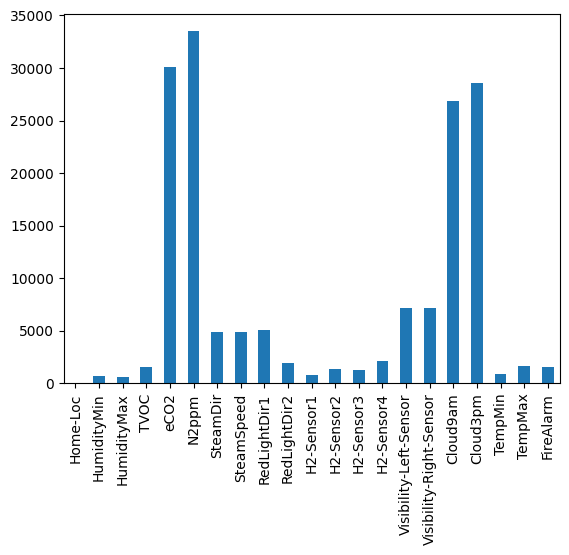
\includegraphics[scale=.45]{./p1-1}
%     \caption{پرسپترون نمودار 1}\label{fig.14}
% \end{figure}



در مواردی که گراف شبکه خواسته شده است، از دو طریق این کار انجام شده است. نمای کلی گراف خروجی تنسوربورد گذاشته شده است. در این ابزار با کلیک بر روی هر قسمت اطلاعات جامعی از شبکه بدست می‌آید. که به عنوان مثال معماری لایه‌ها با تابع دیگری در گزارش آورده شده است.

\section{سوال اول}

\subsection{تخمین مقادیر گم‌شده}

روش‌های متعددی برای این قسمت وجود دارد که در ادامه به معرفی برخی از آن‌ها می‌پردازیم:

\begin{itemize}
    \item حذف سطر یا ستون‌ها: در این روش سطر و ستون‌هایی که شامل مقادیر گم‌شده هستند با شروطی می‌توانند حذف شوند.
    \item حذف سطر یا ستون‌هایی که درصد قابل توجهی از آن داده گم‌شده است.
    \item حذف یا نگهداری سطر یا ستون‌هایی که از یک مقدار حد آستانه بیشتر یا کمتر مقادیر گم‌شده دارند.
    \item همچنین می‌توان بر اساس زیر مجموعه‌ای از سطر یا ستون‌ها این مقادیر را حذف کرد.
    \item اما بعضی اوقات این مقادیر محدود هستند و ترجیح بر آن خواهد بود که سطرها یا ستون‌ها حذف نشوند. یک روش برای این کار پر کردن این مقادر با مقادیر ثابت خواهد بود که برای هر نوع داده‌ای می‌تواند مورد استفاده قرار گیرد.
    \item روش دیگر مورد استفاده برای پر کرده داده‌ها، استفاده از میانگین، میانه یا مد خواهد بود که می‌تواند مفید واقع شود.
    \item روش دیگر استفاده از مقدار قبلی یا بعدی در یک ستون مشخص است (مفید برای داده‌های سری زمانی).
\end{itemize}

برای قسمت پیش پردازش به طور کلی بدین صورت عمل کردیم که اگر سطری بیش از 14 مقدار گم‌شده داشت، حذف شد. بعد از آن میانگین را برای مقادیر گم‌شده عددی و بیشترین برچسب هر ستون برای مقادیر گم‌شده دسته‌بندی را جایگذاری کردیم. در شکل تعداد مقادیر گم‌شده قبل از حذف و در شکل تعداد مقادیر گم‌شده مشاهده می‎‌شود. همچنین در شکل مقادیر جایگذاری‌شده مشاهده می‌شود.

\begin{figure}[!h]
    \centering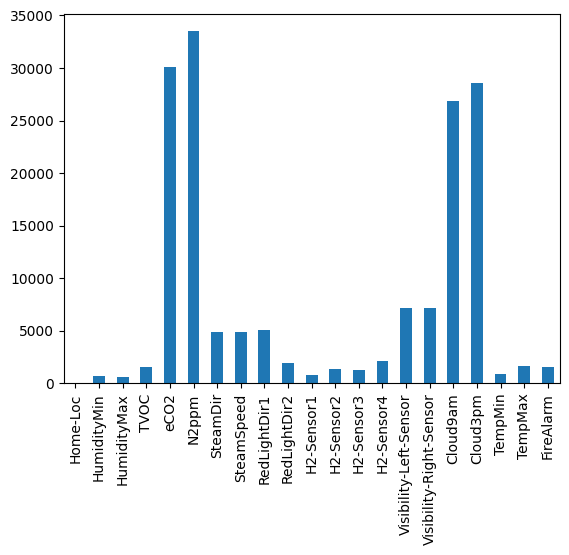
\includegraphics[scale=.55]{./p1-1}
    \caption{تعداد مقادیر گم‌شده برای هر ویژگی قبل از این پیش پردازش}\label{fig.11}
\end{figure}


\begin{figure}[!h]
    \centering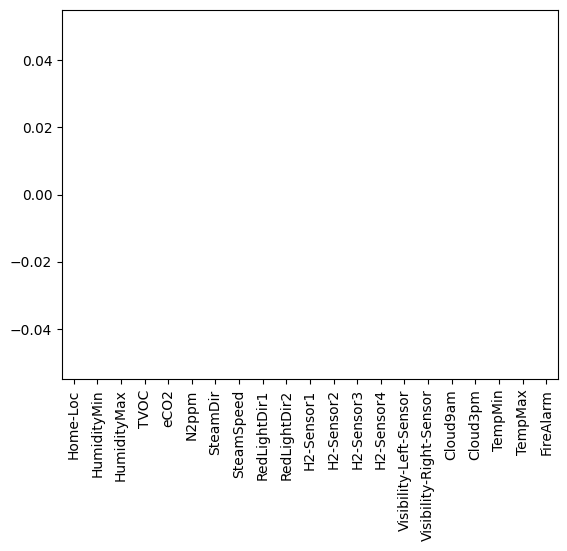
\includegraphics[scale=.55]{./p1-2}
    \caption{تعداد مقادیر گم‌شده برای هر ویژگی بعد از انجام این قسمت}\label{fig.12}
\end{figure}

\begin{figure}[!h]
    \centering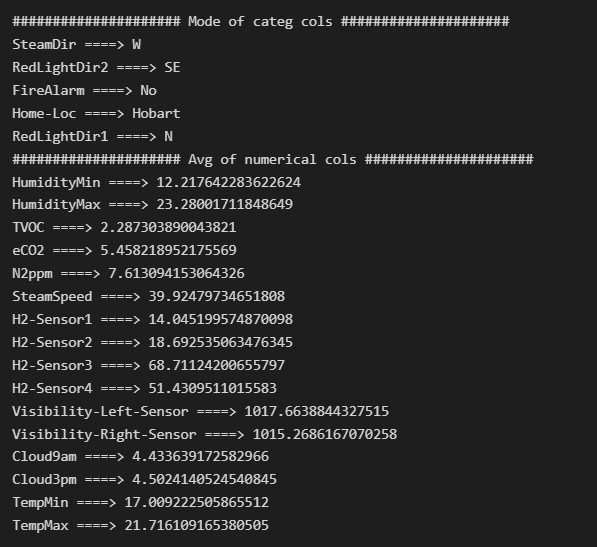
\includegraphics[scale=.55]{./p1-3}
    \caption{مقادیر جایگذاری شده برای مقادیر گم‌شده}\label{fig.13}
\end{figure}



\subsection{نرمال‌سازی}
در آزمایش‌های متعدد دیده شده‌است که مدل‌ها در برابر مجموعه داده‌ای که نرمال‌سازی شده‌است، عملکرد بهتری از خود نشان داده‌اند. به طور کلی این اتفاق زمانی می‌افتد که مقیاس ویژگی‌های عددی یکسان نباشد. به عبارت دیگر، اگر یک ویژگی داشته باشیم که مقدار زیادی از ویژگی دیگر بزرگتر باشد، به طور خودکار ویژگی بزرگتر تاثیر بیشتری در مدل خواهد داشت (مثل درآمد و سن). با نرمال‌سازی تاثیر این دو یکی خواهد شد. پس هدف انتقال تمام ویژگی‌های عددی به یک محدوده خاص است. در این مجموعه داده به عنوان مثال \lr{Visibility} ها مقادیر بزرگتری دارند.

\subsection{تبدیل ویژگی گسسته به عددی}
\begin{itemize}
    \item \lr{Integer Encoding}
    \item \lr{One Hot Encoding}
    \item \lr{Learned Embedding}
\end{itemize}
در این قسمت از روش \lr{One Hot Encoding} استفاده شد. در این روش هر برچسب به یک بردار دودویی تبدیل می‌شود. برای هر داده بررسی می‌شود که آیا این برچسب موجود است یا خیر. پس به ازای هر برچسب ستون (ویژگی) جدید به مجموعه داده اضافه می‌شود.
\\
این روش بدین دلیل انتخاب شد که تضمین می‌کند که مدل به بعضی برچسب‌ها ارزش متفاوتی نمی‌دهد. به عنوان مثال، مقدار 8 بزرگتر از مقدار 1 است، اما این باعث نمی‌شود که 8 از 1 مهم‌تر باشد. همین امر در مورد کلمات صادق است: ارزش جهت‌ها باهم برابر است.


\subsection{حذف داده‌های پرت}

داده پرت، داده ایست که در یک نمونه تصادفی از یک جامعه، فاصله‌ای غیرعادی با مقادیر دیگر دارد. شناسایی داده‌های پرت دارای اهمیت است زیرا ممکن است نشان‌دهنده داده‌های بد باشد، و مدل را دچار انحراف کند. راه‌های شناسایی داده‌های پرت مبتی بر سه روش هستند:

\begin{itemize}
    \item روش‌های آماری: شناسایی با تجزیه و تحلیل بصری داده‌های تک متغیره با استفاده از \lr{Boxplots}، نمودارهای پراکنده می‌تواند به یافتن مقادیر پرت در داده‌ها کمک کند. با فرض توزیع نرمال، 68 درصد داده‌ها در یک طول انحراف استاندارد، 95 درصد در طول دو انحراف استاندارد و 99.7 در سه انحراف استاندارد از میانگین قرار می‌گیرند. با این فروض با درنظر گرفتن فاصله بین چارک اول و سوم، داده‌های با فاصله کمتر از تفریق این فاصله از چارک اول و همچنین بیشتر از جمع این فاصله با چارک سوم را می‌توان به عنوان داده پرت در نظر گرفت.
    \item روش‌های مجاورت: روش‌های مبتنی بر مجاورت، تکنیک‌های خوشه‌بندی را برای شناسایی خوشه‌ها در داده‌ها و یافتن مرکز هر خوشه به کار می‌گیرند. روش بدین صورت است که یک آستانه ثابت می‌شود و فاصله هر نقطه داده از مرکز خوشه ارزیابی می‌شود و سپس نقاط داده پرت حذف می‌شود. یکی از چالش‌ها تعیین آستانه خواهد بود. دو نوع مبتنی بر فاصله و چگالی (\lr{kmean}) را داراست.
    \item روش‌های تصویری: روش‌های پروجکشن از تکنیک‌هایی مانند \lr{PCA} برای مدل‌سازی داده‌ها در یک زیرفضای با ابعاد پایین‌تر با استفاده از همبستگی‌های خطی استفاده می‌کنند. پس از آن، فاصله هر نقطه داده تا صفحه ای که متناسب با فضای فرعی است محاسبه می‌شود. سپس می‌توان از این فاصله برای یافتن نقاط پرت استفاده کرد.
\end{itemize}


اما شناسایی داده‌های پرت با \lr{kmean} بدین صورت خواهد بود که با استفاده از یک مقدار برای \lr{k} بعد از خوشه‌بندی، فاصله هر داده از مرکز را حساب کرده و داده‌های بیشتر از یک آستانه مشخص را به عنوان داده پرت درنظر گرفته و آن حذف می‌شود. در این بخش مقدار 2 برای \lr{k} و آستانه 70 تعداد  438 نمونه حذف شدند.


\section{سوال دوم}

شبکه عمیقی که برای این بخش باید طراحی شود، یک تک پرسپترون خواهد بود. ورودی این تک پرسپترون تمام ویژگی‌ها و خروجی آن هم برچسب مورد نظر خواهد بود. اگر یک تک پرسپترون درجه اول داشته باشیم، میتوان مسائل جداپذیر خطی را حل کند. این بدان دلیل است که تنها یک ضریب در ویژگی‌ها ضرب خواهد شد و با یک مقدار ثابت جمع خواهد شد. بدین ترتیب یک مدل خطی خواهیم داشت. درواقع با یک شبکه تک لایه می‌توان به این دانش رسید.

همانطور که مشاهده می‌شود صحت از 85 درصد بیشتر نمی‌شود. این مسئله بوضوع جدا پذیر خطی نیست. به بیان دیگر پرسپترون نتوانست به 100 درصد صحت برسد.

\begin{figure}[!h]
    \centering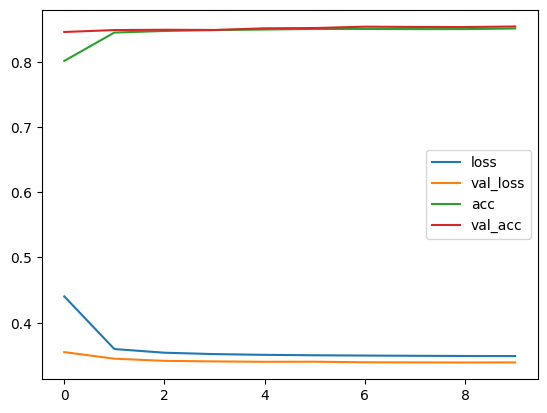
\includegraphics[scale=.55]{./p2-1}
    \caption{خطا و صحت پرسپترون}\label{fig.21}
\end{figure}


\section{سوال سوم}


در این قسمت 96 شبکه عصبی (شامل صفر لایه پنهان تا 7 لایه پنهان) آموزش داده شد (حدود 50 دقیقه). فرض‌هایی که در تمام این شبکه‌های عصبی یکسان بود به صورت زیر است:

\begin{table}[h!]
    \centering
    \begin{tabular}{|c|c|c|c|c|c|c|}
    \hline
    آموزشی داده‌های نسبت & اعتبارسنجی داده‌های نسبت & پنهان فعالیت تابع & خروجی فعالیت تابع & دسته اندازه & ای‌پاک \\ \hline
     70 & 10 & \lr{relu} & \lr{sigmoid} & 64 & 10    \\ \hline
    \end{tabular}
\end{table}


اندازه دسته بهتر بود برابر 16 یا 32 قرار داده می‌شد اما آموزش شبکه‌های عصبی بسیار زمان بر بود، به همین دلیل اندازه دسته برابر 64 گذاشته شد ب این حال آموزش 96 شبکه حدود 50 دقیقه زمان برد.

همچنین تعداد نورون لایه‌های پنهان بر اساس لیستی شامل 64، 128، 192 و 256 بود. در شبکه‌های عصبی با یک و دو لایه تمام حالت‌ها درنظر گرفته شدند، اما در شبکه‌های سه لایه تا 7 لایه به 15 انتخاب تصادفی از تمام حالت‌های ممکن بسنده شد. در ادامه جدولی شامل تمام شبکه‌ها به همراه معماری و همچنین صحت داده‌های آموزشی و اعتبارسنجی آورده شده است:

%#################################################################################################
% \begin{table}[h!]
%     \centering
    \begin{longtable}{|c|c|c|c|c|}
        \hline
        شماره             & پنهان لایه تعداد & شبکه معماری & آموزش مجموعه صحت & اعتبارسنجی مجموعه صحت \\ \hline
        1 & 0 &  - & $85.11$ & $85.22$ \\ \hline
        2 & 1 &  64 & $87.58$ & $85.99$ \\ \hline
        3 & 1 &  128 & $88.12$ & $86.01$ \\ \hline
        4 & 1 &  192 & $88.58$ & $86.07$ \\ \hline
        5 & 1 &  256 & $88.51$ & $86.13$ \\ \hline
        6 & 2 &  64-64 & $88.59$ & $86.14$ \\ \hline
        7 & 2 &  64-128 & $88.63$ & $86.04$ \\ \hline
        8 & 2 &  64-192 & $88.83$ & $85.93$ \\ \hline
        9 & 2 &  64-256 & $88.97$ & $85.82$ \\ \hline
        10 & 2 &  128-64 & $90.06$ & $85.25$ \\ \hline
        11 & 2 &  128-128 & $89.67$ & $85.86$ \\ \hline
        12 & 2 &  128-192 & $89.97$ & $85.52$ \\ \hline
        13 & 2 &  128-256 & $90.86$ & $84.47$ \\ \hline
        14 & 2 &  192-64 & $90.76$ & $85.65$ \\ \hline
        15 & 2 &  192-128 & $91.23$ & $85.45$ \\ \hline
        16 & 2 &  192-192 & $91.64$ & $85.4$ \\ \hline
        17 & 2 &  192-256 & $91.93$ & $85.03$ \\ \hline
        18 & 2 &  256-64 & $91.28$ & $85.28$ \\ \hline
        19 & 2 &  256-128 & $91.27$ & $85.76$ \\ \hline
        20 & 2 &  256-192 & $92.15$ & $85.06$ \\ \hline
        21 & 2 &  256-256 & $92.4$ & $85.03$ \\ \hline
        22 & 3 &  192-192-128 & $93.4$ & $83.87$ \\ \hline
        23 & 3 &  64-64-256 & $89.5$ & $85.58$ \\ \hline
        24 & 3 &  128-256-192 & $93.12$ & $84.15$ \\ \hline
        25 & 3 &  192-64-128 & $91.78$ & $84.85$ \\ \hline
        26 & 3 &  64-128-192 & $90.2$ & $85.58$ \\ \hline
        27 & 3 &  192-192-192 & $93.5$ & $84.36$ \\ \hline
        28 & 3 &  192-256-64 & $93.19$ & $84.87$ \\ \hline
        29 & 3 &  192-64-256 & $92.48$ & $84.73$ \\ \hline
        30 & 3 &  128-128-64 & $91.65$ & $85.25$ \\ \hline
        31 & 3 &  128-64-256 & $91.06$ & $85.01$ \\ \hline
        32 & 3 &  256-64-192 & $92.23$ & $84.44$ \\ \hline
        33 & 3 &  256-128-192 & $93.23$ & $84.76$ \\ \hline
        34 & 3 &  192-128-192 & $93.33$ & $84.32$ \\ \hline
        35 & 3 &  64-256-192 & $90.69$ & $85.09$ \\ \hline
        36 & 3 &  192-128-64 & $92.28$ & $85.07$ \\ \hline
        37 & 4 &  256-192-128-256 & $94.16$ & $84.36$ \\ \hline
        38 & 4 &  192-192-192-64 & $93.43$ & $84.85$ \\ \hline
        39 & 4 &  64-64-64-128 & $89.64$ & $85.28$ \\ \hline
        40 & 4 &  64-64-128-256 & $89.83$ & $85.01$ \\ \hline
        41 & 4 &  192-128-64-192 & $92.82$ & $84.94$ \\ \hline
        42 & 4 &  256-128-192-256 & $93.33$ & $84.76$ \\ \hline
        43 & 4 &  128-64-64-64 & $91.04$ & $85.43$ \\ \hline
        44 & 4 &  256-192-128-256 & $94.08$ & $84.32$ \\ \hline
        45 & 4 &  128-64-192-192 & $91.69$ & $84.73$ \\ \hline
        46 & 4 &  192-256-128-256 & $93.32$ & $84.66$ \\ \hline
        47 & 4 &  192-128-192-192 & $93.48$ & $84.2$ \\ \hline
        48 & 4 &  128-256-256-256 & $93.18$ & $84.51$ \\ \hline
        49 & 4 &  192-192-192-192 & $93.97$ & $84.04$ \\ \hline
        50 & 4 &  64-128-128-64 & $90.02$ & $85.16$ \\ \hline
        51 & 4 &  256-256-192-128 & $93.97$ & $84.67$ \\ \hline
        52 & 5 &  256-192-256-256-128 & $93.84$ & $85.09$ \\ \hline
        53 & 5 &  256-64-192-256-64 & $92.47$ & $84.5$ \\ \hline
        54 & 5 &  192-64-192-64-192 & $92.14$ & $84.94$ \\ \hline
        55 & 5 &  192-128-128-128-64 & $93.05$ & $84.48$ \\ \hline
        56 & 5 &  128-64-128-64-128 & $91.29$ & $84.48$ \\ \hline
        57 & 5 &  64-192-192-128-64 & $90.75$ & $85.15$ \\ \hline
        58 & 5 &  256-256-256-128-64 & $94.47$ & $83.75$ \\ \hline
        59 & 5 &  128-256-256-64-64 & $92.26$ & $83.98$ \\ \hline
        60 & 5 &  64-64-256-128-128 & $90.33$ & $85.03$ \\ \hline
        61 & 5 &  192-128-256-192-192 & $93.49$ & $84.6$ \\ \hline
        62 & 5 &  128-256-64-192-192 & $92.12$ & $85.92$ \\ \hline
        63 & 5 &  128-64-256-128-64 & $91.21$ & $84.66$ \\ \hline
        64 & 5 &  192-256-256-256-192 & $94.05$ & $83.86$ \\ \hline
        65 & 5 &  256-256-64-128-192 & $93.91$ & $84.55$ \\ \hline
        66 & 5 &  64-256-192-64-128 & $91.04$ & $85.19$ \\ \hline
        67 & 6 &  256-128-64-192-64-128 & $93.04$ & $85.27$ \\ \hline
        68 & 6 &  64-256-64-192-192-64 & $90.73$ & $84.97$ \\ \hline
        69 & 6 &  192-256-64-192-256-192 & $92.31$ & $84.72$ \\ \hline
        70 & 6 &  192-192-256-256-256-256 & $93.75$ & $84.48$ \\ \hline
        71 & 6 &  64-128-256-128-256-256 & $90.67$ & $85.09$ \\ \hline
        72 & 6 &  64-192-128-128-192-128 & $90.14$ & $85.31$ \\ \hline
        73 & 6 &  64-128-192-64-64-192 & $90.64$ & $84.72$ \\ \hline
        74 & 6 &  192-64-128-64-256-192 & $91.71$ & $85.18$ \\ \hline
        75 & 6 &  64-128-256-256-192-64 & $90.41$ & $85.42$ \\ \hline
        76 & 6 &  64-256-128-128-128-256 & $91.0$ & $84.39$ \\ \hline
        77 & 6 &  256-256-64-64-128-64 & $93.63$ & $84.15$ \\ \hline
        78 & 6 &  128-64-128-64-64-256 & $91.58$ & $85.12$ \\ \hline
        79 & 6 &  256-128-64-64-256-128 & $92.9$ & $85.01$ \\ \hline
        80 & 6 &  64-192-256-64-64-64 & $90.85$ & $84.75$ \\ \hline
        81 & 6 &  128-64-128-64-256-64 & $91.3$ & $85.31$ \\ \hline
        82 & 7 &  192-192-256-128-192-256-256 & $92.47$ & $85.18$ \\ \hline
        83 & 7 &  256-256-64-128-256-192-192 & $94.05$ & $84.87$ \\ \hline
        84 & 7 &  64-128-128-64-192-128-192 & $90.2$ & $84.97$ \\ \hline
        85 & 7 &  128-192-64-64-256-192-192 & $92.0$ & $84.12$ \\ \hline
        86 & 7 &  128-128-64-192-64-64-128 & $91.24$ & $85.71$ \\ \hline
        87 & 7 &  64-256-128-192-128-64-192 & $90.69$ & $85.76$ \\ \hline
        88 & 7 &  192-256-256-128-128-128-192 & $93.35$ & $84.58$ \\ \hline
        89 & 7 &  192-256-256-192-128-256-128 & $93.29$ & $84.2$ \\ \hline
        90 & 7 &  192-256-128-64-256-128-192 & $92.84$ & $84.85$ \\ \hline
        91 & 7 &  256-128-192-128-256-192-192 & $93.04$ & $84.73$ \\ \hline
        92 & 7 &  256-128-64-192-64-128-128 & $92.4$ & $84.11$ \\ \hline
        93 & 7 &  192-192-256-128-192-256-256 & $93.44$ & $84.38$ \\ \hline
        94 & 7 &  128-256-64-128-192-192-192 & $92.26$ & $85.53$ \\ \hline
        95 & 7 &  256-64-192-64-128-192-64 & $92.38$ & $84.78$ \\ \hline
        96 & 7 &  64-128-192-256-192-128-192 & $90.54$ & $85.43$ \\ \hline
    \end{longtable}
    % \end{table}
    %#################################################################################################




تفاسیر متعددی می‌توان برروی این جدول ارائه داد. به طور کلی با افزایش لایه‌ها به علت پیچیده شدن مدل (افزایش پارامترها)، بیش برازش اتفاق می‌افتد (افزایش صحت آموزش و کاهش صحت اعتبارسنجی). بیشترین صحت مجموعه اعتبارسنجی مربوط به شبکه‌های 6 و 5 و بعد از آن به شبکه‌های 4، 7 و 3 مربوط می‌شود. تمام این شبکه‌ها مربوط به شبکه‌های با 1 و 2 لایه پنهان هستند. البته در موارد انتخابی اختلاف مقادیر صحت آموزشی و اعتبار سنجی نیز لحاظ شده‌است که کم باشد. پس با موارد بیشتری را برای این شبکه‌های با 1 و 2 لایه لحاظ می‌کنیم. در ادامه نتایج آموزش 21 شبکه با فرض‌های اولیه آورده شده است. بدیهی است که موارد مشترک با جدول قبل ممکن است نتایج متفاوتی داشته باشند.


\begin{longtable}{|c|c|c|c|c|}
    \hline
    شماره             & پنهان لایه تعداد & شبکه معماری & آموزش مجموعه صحت & اعتبارسنجی مجموعه صحت \\ \hline
    1 & 1 & 16  & $86.68$ & $86.25$ \\ \hline
    2 & 1 & 32  & $86.9$ & $86.11$ \\ \hline
    3 & 1 & 64  & $87.57$ & $86.02$ \\ \hline
    4 & 1 & 128  & $88.13$ & $85.99$ \\ \hline
    5 & 1 & 256  & $88.79$ & $85.82$ \\ \hline
    6 & 2 & 16-16  & $86.85$ & $86.1$ \\ \hline
    7 & 2 & 16-32  & $86.75$ & $86.13$ \\ \hline
    8 & 2 & 16-64  & $86.94$ & $86.71$ \\ \hline
    9 & 2 & 16-128  & $86.94$ & $85.73$ \\ \hline
    10 & 2 & 32-16  & $87.61$ & $85.98$ \\ \hline
    11 & 2 & 32-32  & $87.41$ & $86.22$ \\ \hline
    12 & 2 & 32-64  & $87.25$ & $86.25$ \\ \hline
    13 & 2 & 32-128  & $87.42$ & $86.25$ \\ \hline
    14 & 2 & 64-16  & $88.26$ & $86.16$ \\ \hline
    15 & 2 & 64-32  & $88.41$ & $86.01$ \\ \hline
    16 & 2 & 64-64  & $88.76$ & $85.83$ \\ \hline
    17 & 2 & 64-128  & $88.81$ & $85.91$ \\ \hline
    18 & 2 & 128-16  & $89.35$ & $85.99$ \\ \hline
    19 & 2 & 128-32  & $89.37$ & $85.28$ \\ \hline
    20 & 2 & 128-64  & $89.62$ & $85.65$ \\ \hline
    21 & 2 & 128-128  & $90.06$ & $85.27$ \\ \hline
\end{longtable}








از این تعداد شبکه عصبی، موارد زیر بهترین نتایج اعتبارسنجی را ارائه کردند:

\begin{longtable}{|c|c|c|c|c|}
    \hline
    شماره             & پنهان لایه تعداد & شبکه معماری & آموزش مجموعه صحت & اعتبارسنجی مجموعه صحت \\ \hline
    8 & 2 & 16-64  & $86.94$ & $86.71$ \\ \hline
    13 & 2 & 32-128  & $87.42$ & $86.25$ \\ \hline
    12 & 2 & 32-64  & $87.25$ & $86.25$ \\ \hline
    1 & 1 & 16  & $86.68$ & $86.25$ \\ \hline

\end{longtable}

توجه در تمام جداول بالا در قسمت معماری شبکه، ترتیب لایه‌ها از راست به چپ است.

پس انتخاب ما شبکه عصبی با دو لایه پنهان با تعداد نورون 16 و 64 خواهد بود. معماری مدل نهایی نیز به صورت زیر است:


\begin{figure}[!h]
    \centering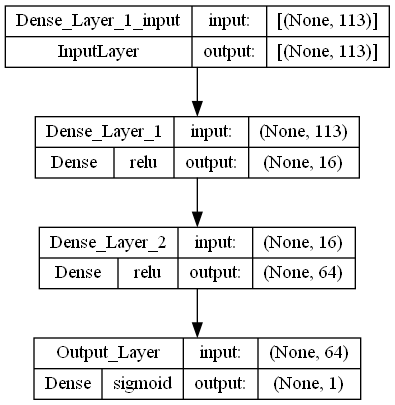
\includegraphics[scale=.55]{./p3-3}
    \caption{معماری مدل نهایی}\label{fig.33}
\end{figure}

در ادامه دو نمودار صحت و خطا بر حسب ای‌پاک (تا 10 ای‌پاک) را برای دو مجموعه اعتبارسنجی و آموزشی می‌بینیم.

\begin{figure}[!h]
    \centering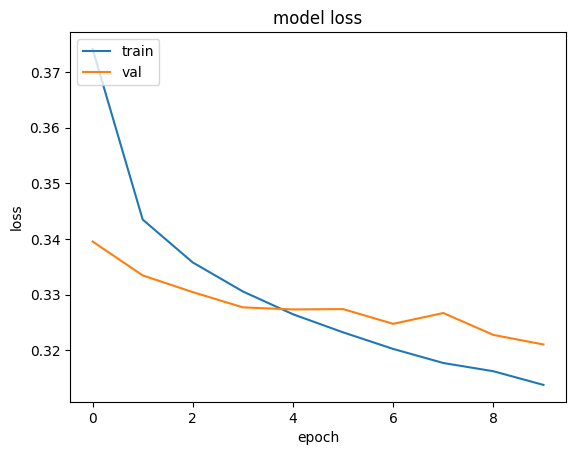
\includegraphics[scale=.55]{./p3-1}
    \caption{نمودار خطا بر اساس ای‌پاک}\label{fig.31}
\end{figure}


\begin{figure}[!h]
    \centering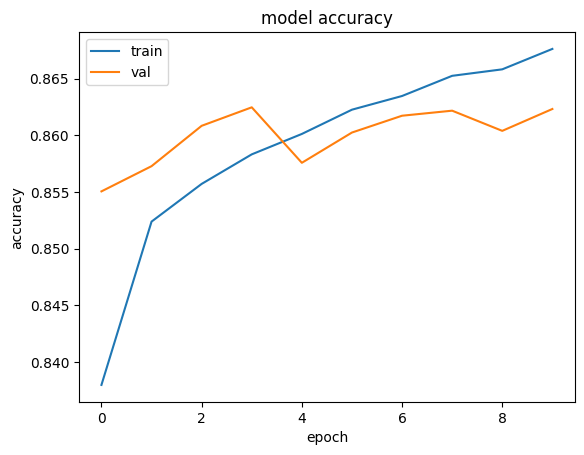
\includegraphics[scale=.55]{./p3-2}
    \caption{نمودار صحت بر اساس ای‌پاک}\label{fig.32}
\end{figure}


گراف شبکه نهایی با ابزار تنسور بورد نیز تولید شد که به شرح زیر است.

\begin{figure}[!h]
    \centering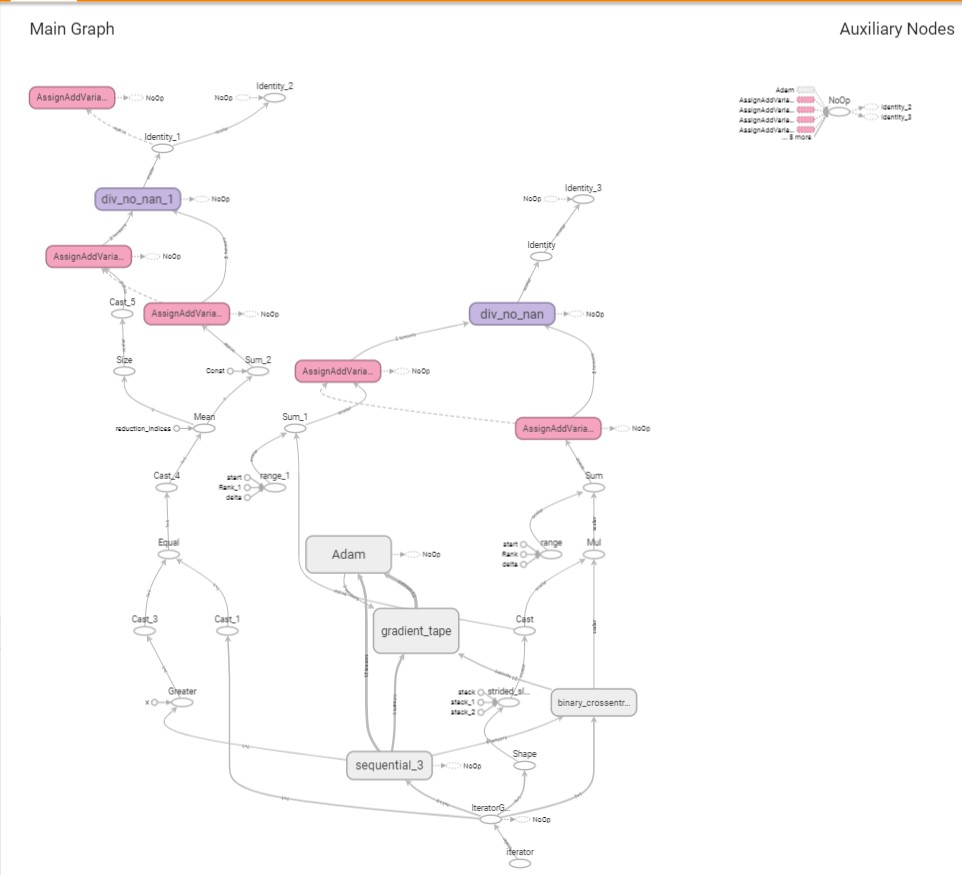
\includegraphics[scale=.55]{./p3-4}
    \caption{گراف شبکه نهایی با ابزار تنسور بورد}\label{fig.34}
\end{figure}




\cleardoublepage

\section{سوال چهارم}


توابع فعالیت با ویژگی غیرخطی بودن نقشی اساسی در شبکه‌های عصبی ایفا می‌کنند. این غیرخطی بودن به شبکه‌های عصبی اجازه می‌دهد تا نمایش‌ها و توابع پیچیده‌ای را آموزش دهند که با یک مدل رگرسیون خطی ساده امکان‌پذیر نیست. درواقع اگر توابع فعالیت نباشند، پیچیده‌ترین شبکه‌ها قابلیت مدل شدن با یک پرسپترون را خواهند داشت. حال نوع این توابع فعالیت برای غیرخطی کردن خروجی بسیار حائز اهمیت است. درواقع این انواع مختلف است که منجر به خروجی‌های متفاوت خواهد شد. همچنین برروی سرعت آموزش مدل هم تاثیرگذار خواهد بود.

در این قسمت 3 نوع تابع فعالیت برای شبکه حاصل سوال 3 (16 و 64 نورون برای لایه‌های اول و دوم) درنظر گرفته شد (با فرض‌های اولیه). که خروجی نهایی در جدول زیر آمده است.

\begin{longtable}{|c|c|c|c|c|}
    \hline
    تابع   & پنهان لایه تعداد & شبکه معماری & آموزش مجموعه صحت & اعتبارسنجی مجموعه صحت \\ \hline
    \lr{tanh} & 2 & 16-64  & $85.96$ & $86.2$ \\ \hline
    \lr{sigmoid} & 2 & 16-64  & $85.51$ & $85.71$ \\ \hline
    \lr{relu} & 2 & 16-64  & $86.94$ & $85.83$ \\ \hline
\end{longtable}


همانطور که مشاهده می‌شود خروجی تا ای‌پاک 10 اختلاف چندانی ندارد اما روند آموزش شبکه‌ها جالب است.

نمودارهای صحت و خطا برای تابع \{tanh} به صورت زیر می‌باشد.


\begin{figure}[!h]
    \centering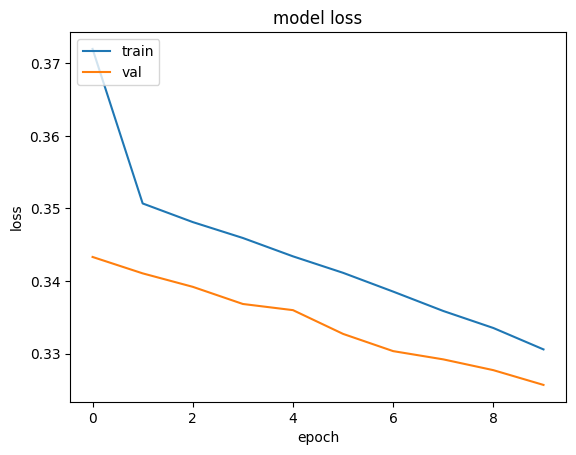
\includegraphics[scale=.55]{./p4-1}
    \caption{نمودار خطا بر اساس ای‌پاک (\lr{tanh})}\label{fig.41}
\end{figure}


\begin{figure}[!h]
    \centering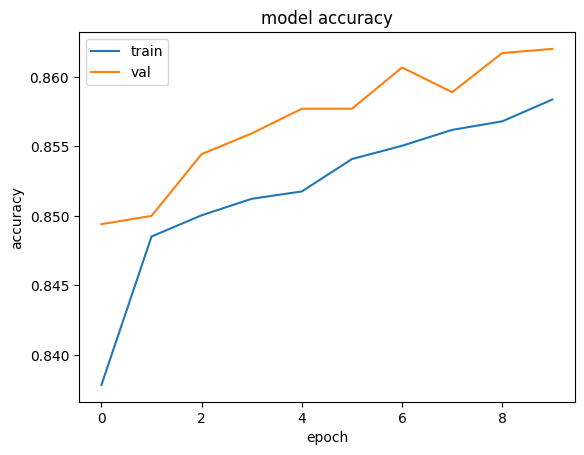
\includegraphics[scale=.55]{./p4-2}
    \caption{نمودار صحت بر اساس ای‌پاک (\lr{tanh})}\label{fig.42}
\end{figure}

\cleardoublepage


نمودارهای صحت و خطا برای تابع \{sigmoid} به صورت زیر می‌باشد.

\begin{figure}[!h]
    \centering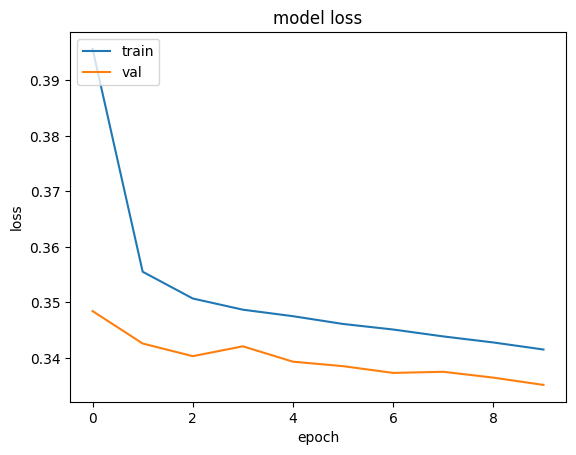
\includegraphics[scale=.55]{./p4-3}
    \caption{نمودار خطا بر اساس ای‌پاک (\lr{sigmoid})}\label{fig.43}
\end{figure}


\begin{figure}[!h]
    \centering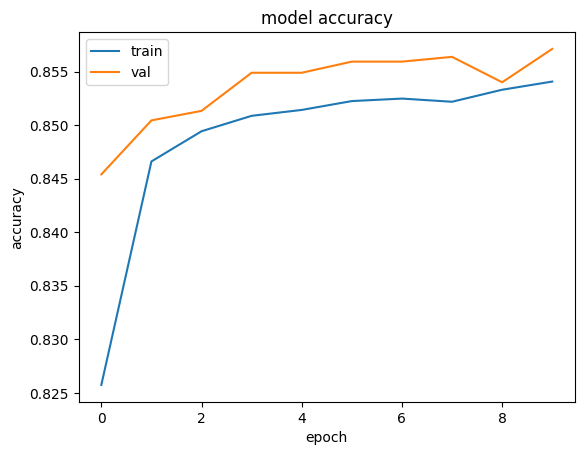
\includegraphics[scale=.55]{./p4-4}
    \caption{نمودار صحت بر اساس ای‌پاک (\lr{sigmoid})}\label{fig.44}
\end{figure}

\cleardoublepage

نمودارهای صحت و خطا برای تابع \{relu} به صورت زیر می‌باشد.

\begin{figure}[!h]
    \centering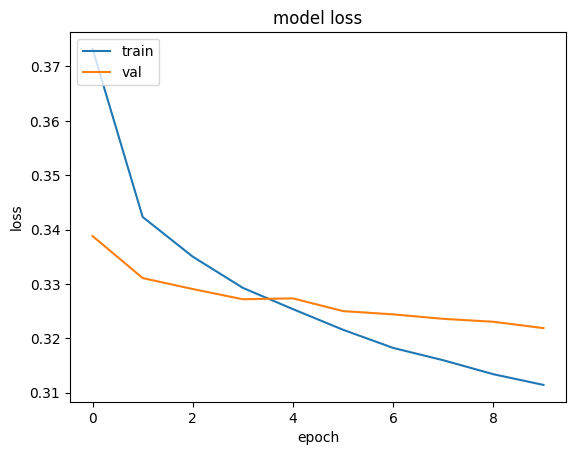
\includegraphics[scale=.55]{./p4-5}
    \caption{نمودار خطا بر اساس ای‌پاک (\lr{relu})}\label{fig.45}
\end{figure}


\begin{figure}[!h]
    \centering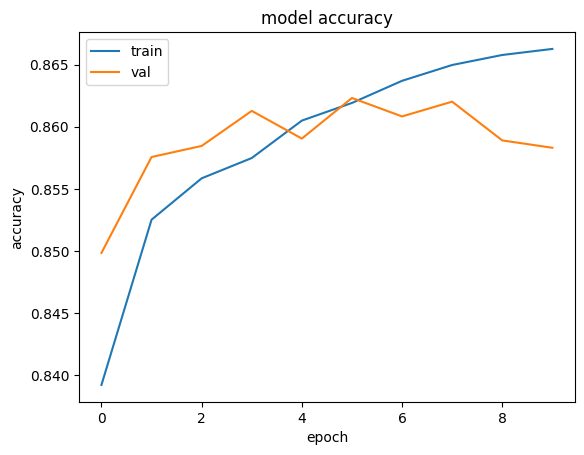
\includegraphics[scale=.55]{./p4-6}
    \caption{نمودار صحت بر اساس ای‌پاک (\lr{relu})}\label{fig.46}
\end{figure}

\cleardoublepage
همانطور که دیده شد، نمودارهای \lr{tanh} و \lr{sigmoid} در صورت ادامه دادن نتایج جالبی خواهند داد. بدین صورت که تا ای‌پاک 10 حتی مقدار صحت اعتبارسنجی بیشتر است و هردو صعودی هستند.
این تفاوت طبیعتا ناشی از تفاوت در نوع توابع فعالیت است. بدین صورت که برای یک شبکه ممکن است یک تابع فعالیت برای لایه‌های پنهانی مناسب باشد ولی برای دیگری نوع دیگری. 
اما در هر صورت تا ای‌پاک 10 بهترین عملکرد مربوط به \lr{tanh} است. البته ممکن است با اجرایی دیگر نتایج متفاوت شود. به عنوان مثال با اجرایی دیگر تا ای‌پاک 20 \lr{sigmoid} بهترین بود.


\section{سوال پنجم}

اندازه‌ دسته در روند آموزش مدل بسیار مهم است. با توجه به آزمایشات انجام شده به این نتیجه رسیدند که افزایش اندازه دسته عملکرد را کاهش می‌دهد (افزایش خطا و کاهش صحت). همچنین گفته شده است که وقتی اندازه دسته افزایش داده می‌شود، باید نرخ یادگیری برای جبران آن تنظیم شود. درواقع بیان می‌شود که تاثیر افزایش اندازه دسته عملکرد مانند کاهش نرخ یادگیری خواهد بود. اما از طرفی با اندازه‌های دسته‌ بزرگ به روند آموزش سرعت داده می‌شود، گاهی اوقات امکان افزایش ۲ برابری در زمان محاسبات وجود دارد.

نتایج تا 10 پیمایش با اندازه‌های دسته 256، 64 و 16 با فرض‌های اولیه سوال سه به صورت زیر خواهد بود:


\begin{longtable}{|c|c|c|c|c|}
    \hline
    دسته اندازه& پنهان لایه تعداد & شبکه معماری & آموزش مجموعه صحت & اعتبارسنجی مجموعه صحت \\ \hline
    256 & 2 & 16-64  & $86.33$ & $85.58$ \\ \hline
    64 & 2 & 16-64  & $86.83$ & $86.2$ \\ \hline
    16 & 2 & 16-64  & $87.34$ & $86.1$ \\ \hline
\end{longtable}


نمودارهای صحت و خطا برای مجموعه آموزشی و اعتبارسنجی و همچنین ماتریس درهم ریختگی برای مجموعه آموزشی برای اندازه دسته 256 به شرح زیر می‌باشد:

\begin{figure}[!h]
    \centering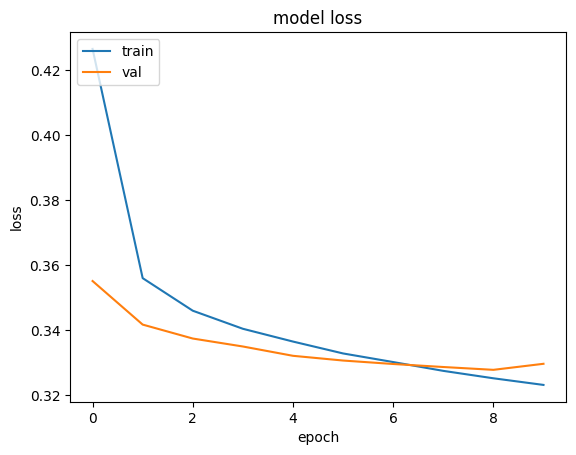
\includegraphics[scale=.55]{./p5-1}
    \caption{نمودار خطا بر اساس ای‌پاک (256)}\label{fig.51}
\end{figure}


\begin{figure}[!h]
    \centering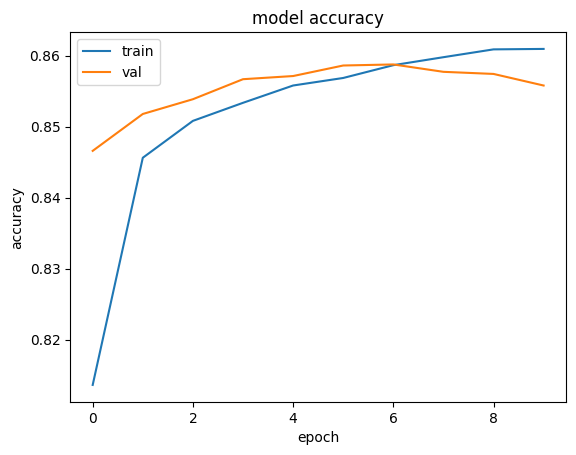
\includegraphics[scale=.55]{./p5-2}
    \caption{نمودار صحت بر اساس ای‌پاک (256)}\label{fig.52}
\end{figure}

\begin{figure}[!h]
    \centering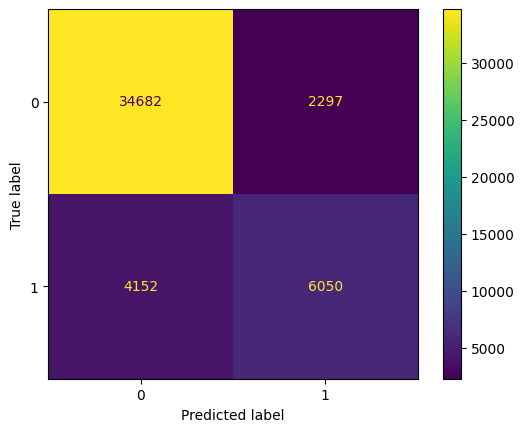
\includegraphics[scale=.55]{./p5-3}
    \caption{ماتریس درهم‌ریختگی بر اساس ای‌پاک (256)}\label{fig.53}
\end{figure}

\cleardoublepage

نمودارهای صحت و خطا برای مجموعه آموزشی و اعتبارسنجی و همچنین ماتریس درهم ریختگی برای مجموعه آموزشی برای اندازه دسته 64  به شرح زیر می‌باشد:

\begin{figure}[!h]
    \centering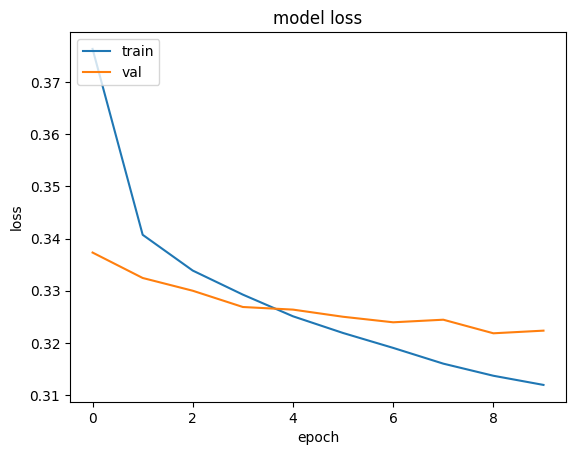
\includegraphics[scale=.55]{./p5-4}
    \caption{نمودار خطا بر اساس ای‌پاک (64)}\label{fig.54}
\end{figure}


\begin{figure}[!h]
    \centering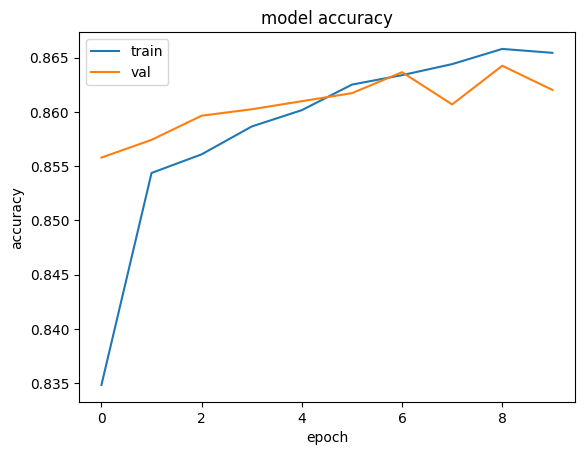
\includegraphics[scale=.55]{./p5-5}
    \caption{نمودار صحت بر اساس ای‌پاک (64)}\label{fig.55}
\end{figure}

\begin{figure}[!h]
    \centering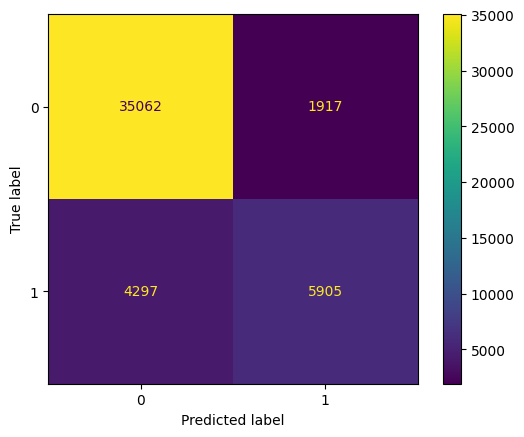
\includegraphics[scale=.55]{./p5-6}
    \caption{ماتریس درهم‌ریختگی بر اساس ای‌پاک (64)}\label{fig.56}
\end{figure}

\cleardoublepage

نمودارهای صحت و خطا برای مجموعه آموزشی و اعتبارسنجی و همچنین ماتریس درهم ریختگی برای مجموعه آموزشی برای اندازه دسته 16 به شرح زیر می‌باشد:

\begin{figure}[!h]
    \centering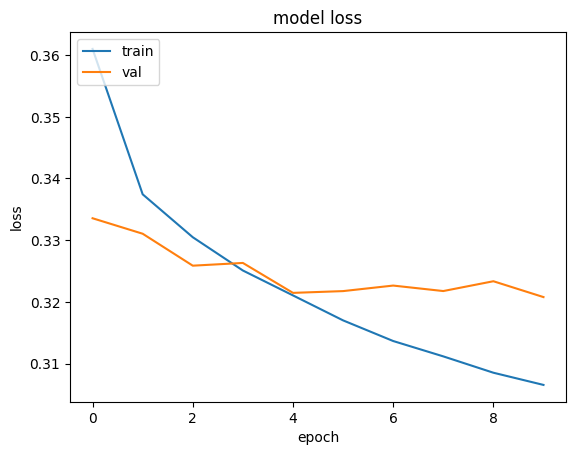
\includegraphics[scale=.55]{./p5-7}
    \caption{نمودار خطا بر اساس ای‌پاک (16)}\label{fig.57}
\end{figure}


\begin{figure}[!h]
    \centering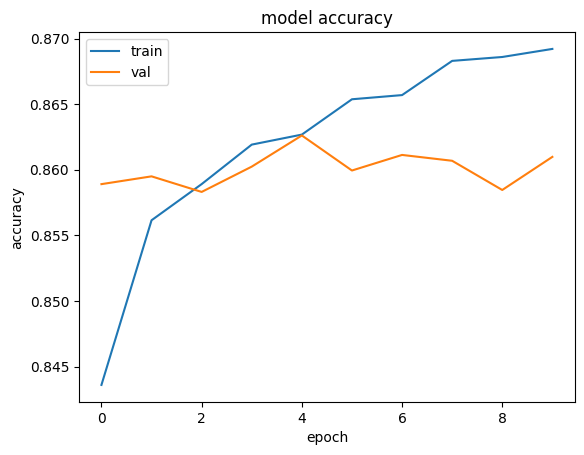
\includegraphics[scale=.55]{./p5-8}
    \caption{نمودار صحت بر اساس ای‌پاک (16)}\label{fig.58}
\end{figure}

\begin{figure}[!h]
    \centering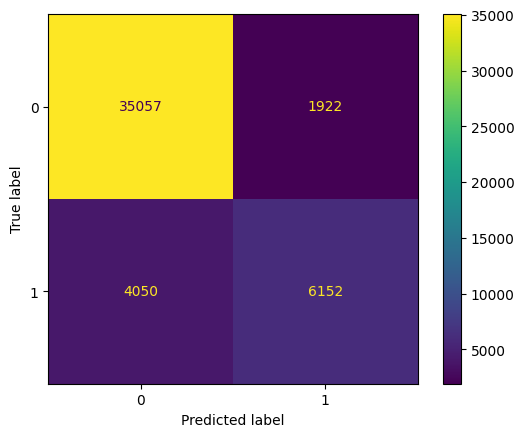
\includegraphics[scale=.55]{./p5-9}
    \caption{ماتریس درهم‌ریختگی بر اساس ای‌پاک (16)}\label{fig.59}
\end{figure}

\cleardoublepage

همانطور که در جدول  جمع‌بندی اندازه دسته مشاهده می‌شود، برای مجموعه آموزش بیش‌ترین مقدار صحت مجموعه آموزشی برای کمترین مقدار اندازه دسته است. این اتفاق در ماتریس‌های درهم‌ریختگی نیز قابل مشاهده است. اما تفسیر نمودارهای صحت و خطا نیز جالب است: همانطور که مشاهده می‌شود به ازای مقادیر مختلف اندازه دسته، ای‌پاک‌هایی که بعد از کاهش صحت مجموعه اعتبارسنجی را داریم متفاوت هستند. این اتفاق با توجه به برابری تاثیر نرخ یادگیری و اندازه دسته است، کاملا صادق است.


\section{سوال ششم}

بیش‌برازش زمانی اتفاق می‌افتد که مدل دارای واریانس بالایی باشد، به‌عنوان مثال، مدل در داده‌های آموزشی به خوبی عمل می‌کند اما در مجموعه تست و اعتبارسنجی عملکرد مناسبی ندارد. به بیان دیگر، مدل وابستگی زیادی به داده‌های آموزشی پیدا می‌کند. این وابستگی به قدری زیاد است که مانع عملکرد مطلوب در مجموعه‌های آموزش ندیده می‌شود.
بیش‌برازش را می‌توان با بررسی صحت و خطا اعتبارسنجی شناسایی کرد. به عنوان مثال خطا اعتبارسنجی معمولاً تا نقطه‌ای کاهش می‌یابد و بعد از آن شروع به افزایش می‌کند. که از این نقطه به بعد مدل دچار بیش‌برازش می‌شود. یکی از راه‌های ایجاد بیش برازش، تولید یک مدل بسیار پیچیده‌تر از نیاز مسئله است. همچنین اگر داده‌های آموزشی کم باشند، این اتفاق خواهد افتاد. 
تکنینک‌های مختلفی برای جلوگیری از بیش‌برازش وجود دارد: 

\begin{itemize}
    \item \lr{Drop out}
    \item \lr{Regularization}
    \item \lr{Early stopping}
\end{itemize}

البته تکنیک‌های دیگری نیز وجود دارند، که در اینجا به 3 تکنیک بسنده شد.

در واقع برای رسیدن به بیش‌برازش باید مدل آموزش داده شود که پارامتر‌های بسیار زیادی داشته باشد، تا صحت بالا و خطای کمی بر روی مجموعه آموزش و در طرف دیگر صحت کم و خطای بالا برای مجموعه تست و اعتبار سنجی بدست بیاید. برای طرحی این قسمت ما از نتایج تولید شده در سوال 3 استفاده می‌کنیم. معماری‌ای انتخاب می‌شود که بیشترین صحت مجموعه آموزشی و کمترین صحت مجموعه اعتبارسنجی را دارا باشد. شبکه 58 با 5 لایه مخفی انتخاب شد. البته می‌توان شبکه‌های با لایه بیشتر نیز انتخاب کرد، اما همین معماری برای این بخش کافی خواهد بود. همچنین برای رخ دادن بیش‌برازش مقدار ای‌پاک را تا 100 افزایش می‌دهیم.

\begin{longtable}{|c|c|c|c|c|}
    \hline
    دسته اندازه& پنهان لایه تعداد & شبکه معماری & آموزش مجموعه صحت & تست مجموعه صحت \\ \hline
    64 & 5 & 256-256-256-128-64  & $99.8$ & $82.1$ \\ \hline
\end{longtable}

نمودارهای صحت و خطا برای مجموعه آموزشی و تست و همچنین ماتریس درهم‌ریختگی برای مجموعه آموزشی و تست به شرح زیر می‌باشد:

\begin{figure}[!h]
    \centering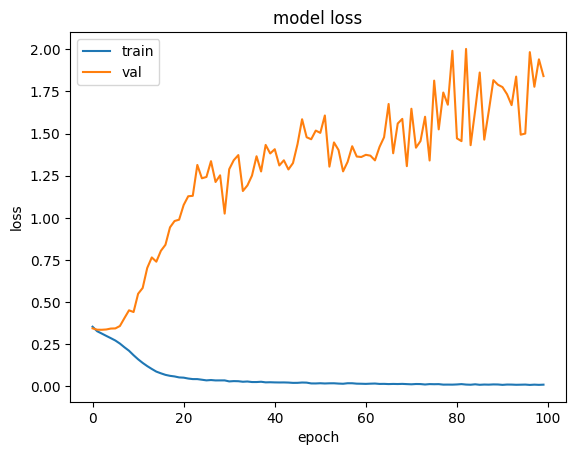
\includegraphics[scale=.55]{./p6-1}
    \caption{نمودار خطا بر اساس ای‌پاک}\label{fig.61}
\end{figure}


\begin{figure}[!h]
    \centering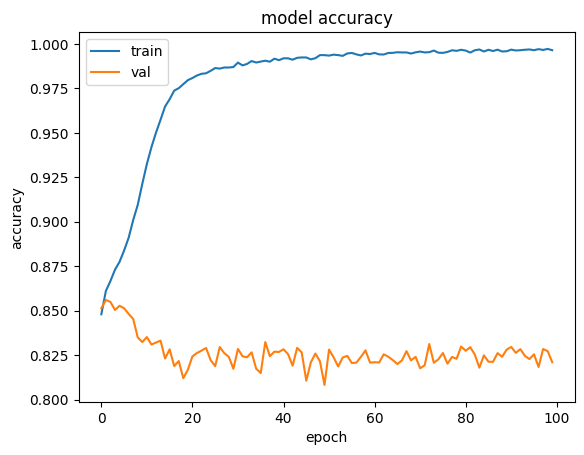
\includegraphics[scale=.55]{./p6-2}
    \caption{نمودار صحت بر اساس ای‌پاک}\label{fig.62}
\end{figure}
\cleardoublepage

\begin{figure}[!h]
    \centering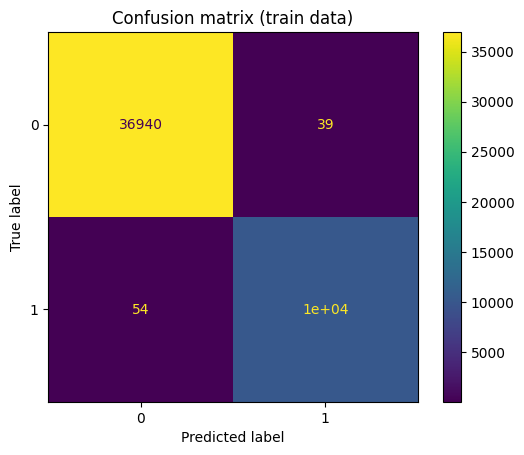
\includegraphics[scale=.55]{./p6-3}
    \caption{ماتریس درهم‌ریختگی مجموعه آموزش بر اساس ای‌پاک}\label{fig.63}
\end{figure}

\begin{figure}[!h]
    \centering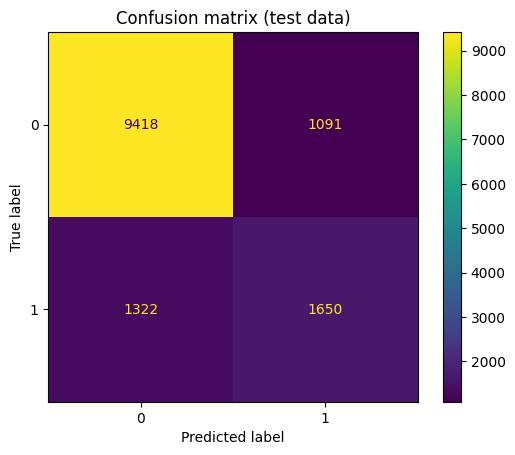
\includegraphics[scale=.55]{./p6-4}
    \caption{ماتریس درهم‌ریختگی مجموعه تست بر اساس ای‌پاک}\label{fig.64}
\end{figure}

\cleardoublepage

\begin{figure}[!h]
    \centering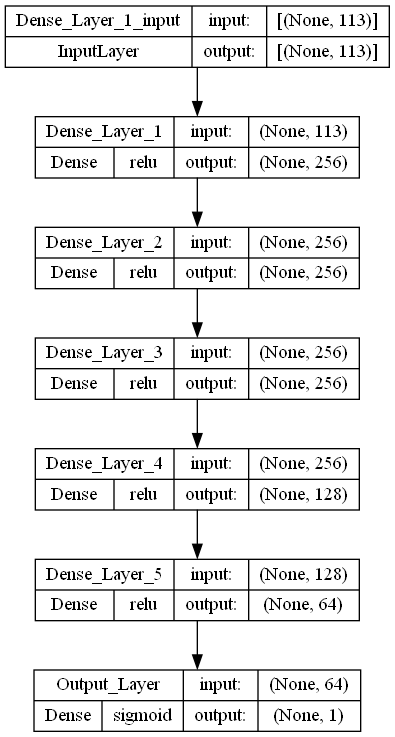
\includegraphics[scale=.55]{./p6-5}
    \caption{گراف شبکه بیش‌برازش شده}\label{fig.65}
\end{figure}

گراف شبکه بیش‌برازش شده با ابزار تنسور بورد نیز تولید شد که به شرح زیر است.


\begin{figure}[!h]
    \centering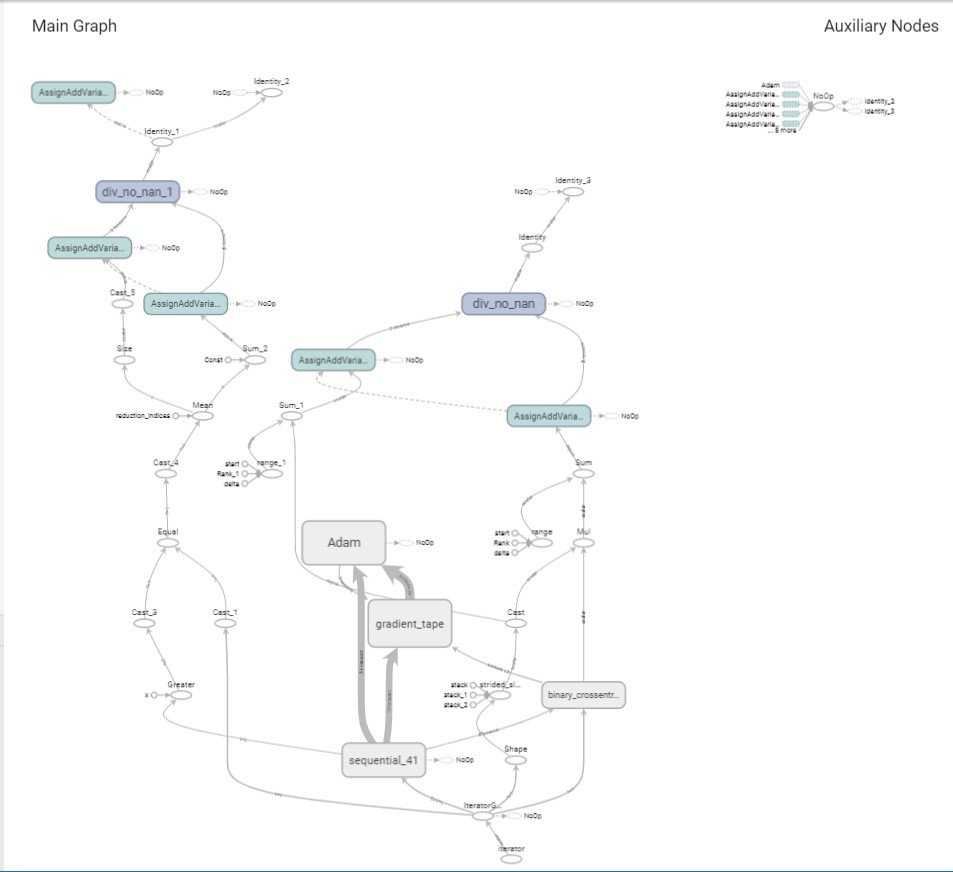
\includegraphics[scale=.55]{./p6-6}
    \caption{گراف شبکه بیش‌برازش شده با ابزار تنسور بورد}\label{fig.66}
\end{figure}



\section{سوال هفتم}

تعمیم‌پذیری به توانایی مدل برای انطباق مناسب با داده‌های جدید و قبلاً دیده نشده (اعتبارسنجی و تست) اشاره دارد. این مفهموم اساساً به این معنی است که مدل ما چقدر در یادگیری از داده‌های داده شده در جاهای دیگر (استفاده واقعی) خوب است. درواقع مدل اساسا برای استفاده در محیط‌های جدید و داده‌های دیده نشده آموزش می‌بیند. پس شبکه باید تعمیم‌پذیر باشد.
برای رسیدن به بهترین تعمیم‌پذیری، مجموعه داده باید به سه قسمت تقسیم شود: مجموعه آموزشی برای آموزش شبکه استفاده می‌شود. خطای این مجموعه داده در طول آموزش به حداقل رسانده می‌شود. مجموعه اعتبارسنجی برای تعیین عملکرد یک شبکه عصبی بر روی الگوهایی که در طول یادگیری آموزش ندیده‌اند استفاده می‌شود. و مجموعه تست که داده‌های محیط جدید درنظر گرفته می‌شوند. یکی از استدلال‌هایی که می‌توان برای تعمیم‌پذیری مدل‌ها ارائه دید، بررسی خطای و صحت مجموعه اعتبارسنجی است. به عنوان مثال صحت این مجموعه باید قابل قبول و نزدیک به مجموعه آموزشی باشد. زمانی که این ختلاف زیاد شود، تعمیم‌پذیری مدل پایین خواهد بود. با این روش می‌توان تعمیم‌پذیری مدل را نشان داد.
برای بهبود تعمیم‌پذیری راه‌هایی که وجود دارند: محدود کردن تعداد وزن‌ها، تقسیم وزن، توقف زودهنگام آموزش، \lr{Regularization}، کاهش وزن و اضافه کردن نویز به ورودی‌ها.


برای طراحی این شبکه از همان نتایج سوال 3 استفاده شد. درواقع بهترین نتیجه سوال 3 که مربوط به شبکه با دو لایه پنهان 16 و 64 نورون بود انتخاب شد و دوباره آموزش داده شد. در این مرحله از آموزش از یک \lr{callback} به نام \lr{early stopping} استفاده شد تا از بیش‌برازش جلوگیری شود.


\begin{longtable}{|c|c|c|c|c|}
    \hline
    شماره             & پنهان لایه تعداد & شبکه معماری & آموزش مجموعه صحت & تست مجموعه صحت \\ \hline
    8 & 2 & 16-64  & $87.27$ & $85.34$ \\ \hline
\end{longtable}
همانطور که مشاهده می‌شود، صحت تست و آموزش نزدیک به هم و همچنین از صحت مناسبی برخوردار است

نمودارهای صحت و خطا برای مجموعه آموزشی و تست و همچنین ماتریس درهم‌ریختگی برای مجموعه آموزشی و تست به شرح زیر می‌باشد:
\cleardoublepage

\begin{figure}[!h]
    \centering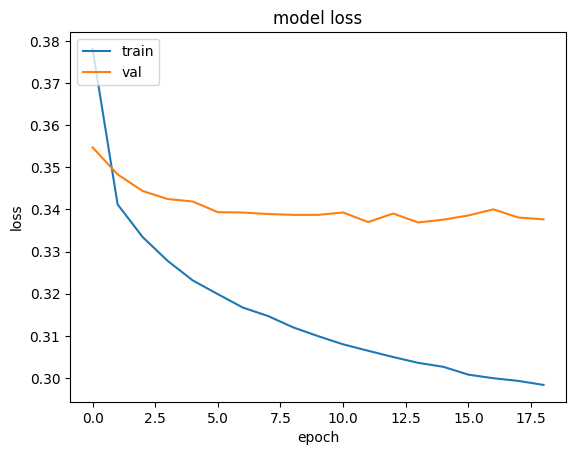
\includegraphics[scale=.55]{./p7-1}
    \caption{نمودار خطا بر اساس ای‌پاک}\label{fig.71}
\end{figure}


\begin{figure}[!h]
    \centering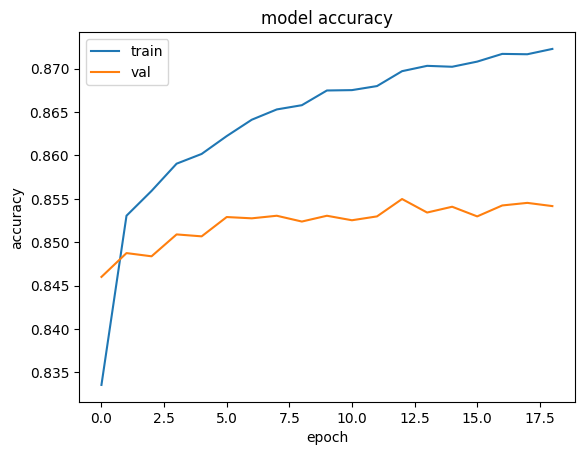
\includegraphics[scale=.55]{./p7-2}
    \caption{نمودار صحت بر اساس ای‌پاک}\label{fig.72}
\end{figure}

\cleardoublepage

\begin{figure}[!h]
    \centering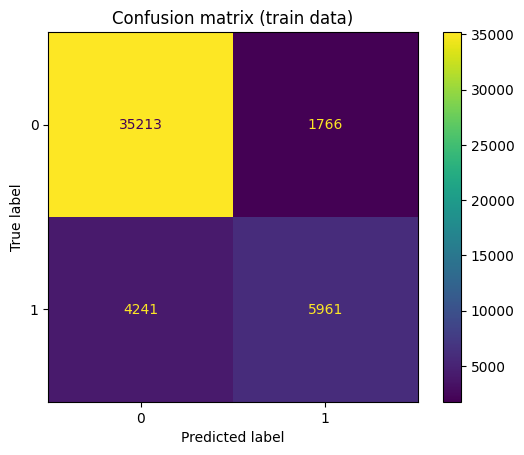
\includegraphics[scale=.55]{./p7-3}
    \caption{ماتریس درهم‌ریختگی مجموعه آموزش بر اساس ای‌پاک}\label{fig.73}
\end{figure}

\begin{figure}[!h]
    \centering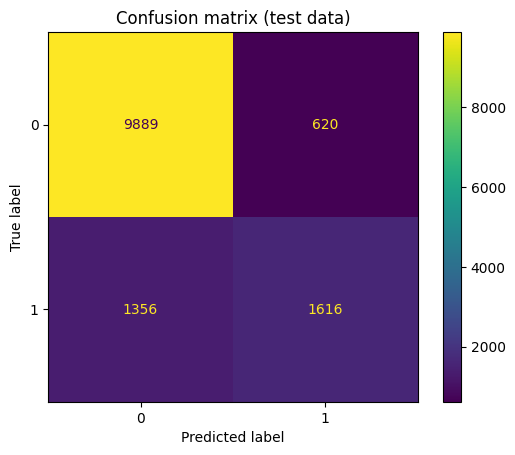
\includegraphics[scale=.55]{./p7-4}
    \caption{ماتریس درهم‌ریختگی مجموعه تست بر اساس ای‌پاک}\label{fig.74}
\end{figure}

\cleardoublepage

\begin{figure}[!h]
    \centering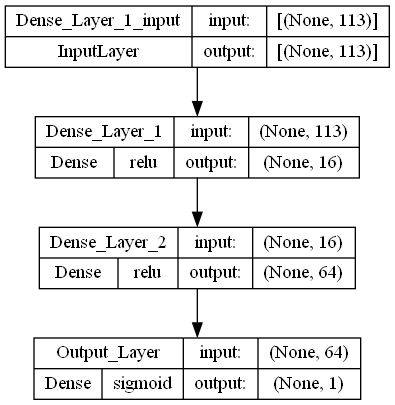
\includegraphics[scale=.55]{./p7-5}
    \caption{گراف شبکه بیش‌برازش شده}\label{fig.75}
\end{figure}

گراف شبکه بیش‌برازش شده با ابزار تنسور بورد نیز تولید شد که به شرح زیر است.


\begin{figure}[!h]
    \centering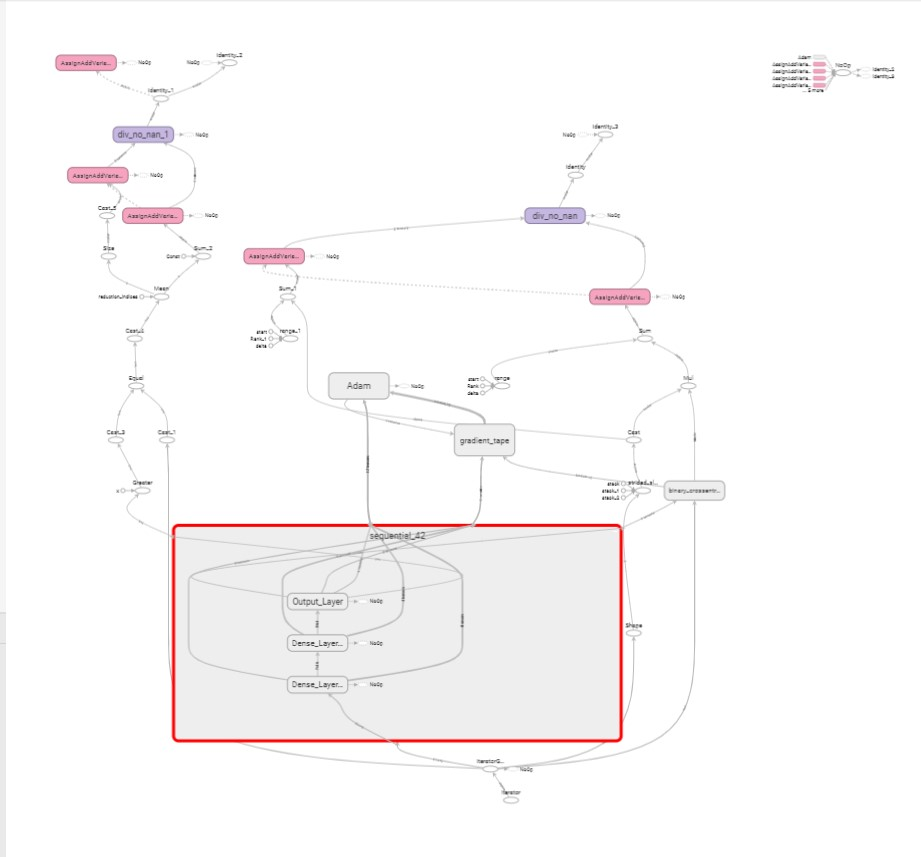
\includegraphics[scale=.55]{./p7-6}
    \caption{گراف شبکه بیش‌برازش شده با ابزار تنسور بورد}\label{fig.76}
\end{figure}
\cleardoublepage

% \section{پیوست}

% \section{ضمیمه}
% برای آشنایی بیشتر با \lr{\LaTeX}، با جست‌و‌جو در اینترنت منابع مفیدی خواهید یافت.

% %\printbibliography[title=منابع]

% \section*{منابع}
% \renewcommand{\section}[2]{}%
% \begin{thebibliography}{99} % assumes less than 100 references
% %چنانچه مرجع فارسی نیز داشته باشید باید دستور فوق را فعال کنید و مراجع فارسی خود را بعد از این دستور وارد کنید

% \begin{LTRitems}

% \resetlatinfont

% % \bibitem{b1} http://mrheidar.ir/courses/operating\_system.html
% \end{LTRitems}

% \end{thebibliography}

\end{document}